\documentclass[10pt,twocolumn]{article}
\usepackage[margin=0.72in]{geometry}
\usepackage{times,microtype,graphicx,booktabs,amsmath,amssymb,url,xcolor}
\usepackage[numbers,sort&compress]{natbib}
\usepackage[hidelinks]{hyperref}
\usepackage{enumitem}
\setlist{nosep,leftmargin=*}
\title{False Is Not One Thing: Matched Probes of Prompted Lies and Epistemic Errors}
\author{Anonymous}
\date{}
\begin{document}
\maketitle

\begin{abstract}
Does a lie detector detect deception, falsehood, uncertainty, or merely the instruction that induced a lie? We cross elicited knowledge with an incentive to misreport on 240 matched TriviaQA questions in Qwen2.5-7B-Instruct. Four neutral samples classify 129 questions as known, 93 as unknown, and 18 as ambiguous. Despite an explicit reward-framed instruction to answer wrongly, only 17/129 known items become false. Of the 116 false outputs under that instruction, only 14.7\% are clean belief-contradicting lies, while 74.1\% arise on low-knowledge items and 11.2\% are ambiguous. A conventional condition probe perfectly separates lie-prompt from truth-prompt examples---but also does so at the final prompt token, before an answer exists. In contrast, a probe trained on actual lying versus correct answers under the \emph{same} lie prompt distinguishes held-out lies from same-pressure honest answers (answer-state AUROC .959) and from hallucinations (.896). A hallucination probe detects held-out low-knowledge errors against known correct answers (AUROC .879), yet barely separates hallucinations from lies (.604, 95\% bootstrap CI [.475, .733]). Thus false-output mixtures are dominated by epistemic failures, and apparently perfect lie detection can be prompt detection; mechanism-sensitive training can help in this narrow setting. Our small, explicit-instruction study is a diagnostic, not evidence about spontaneous strategic deception.
\end{abstract}

\section{Introduction}
Factual error and deception have different safety implications. A system that lacks an answer needs uncertainty estimation or retrieval; one that knows an answer but strategically misreports it needs monitoring of the belief--statement mismatch. Collapsing both into ``false'' makes a detector's success hard to interpret. This matters especially for activation probes: excellent discrimination can arise from a pressure prompt, topic, or uncertainty state without representing deception.

MASK formalized the behavioral separation between accuracy (belief versus ground truth) and honesty (statement versus elicited belief) \citep{ren2025mask}. Liars' Bench broadened lie types and showed incomplete detector transfer \citep{kretschmar2025liars}; belief-verified model organisms sharpened the same concern \citep{cooney2026did}. Yet the elementary false-versus-false contrast remains under-measured: for the same model and matched factual questions, what fraction of false outputs are low-knowledge errors versus knowledge-contradicting reports, and do linear detectors distinguish them?

We make three contributions. First, we instantiate a $3\times3$ behavioral design: elicited knowledge (known/ambiguous/unknown) crossed with neutral, lie-incentive, and incentive-resistance prompts. Second, we report the yield and composition of false outputs rather than treating every lie instruction as a lie. Third, we evaluate condition, hallucination, and same-prompt outcome probes at prompt and answer positions. The central negative finding is that high in-distribution lie-prompt performance is uninformative when the label is readable before generation.

\section{Related Work}
\paragraph{Honesty and deception.}
MASK separates model belief from report using neutral elicitation and pressure \citep{ren2025mask}. Linear probes trained on contrastive honesty instructions can attain AUROCs above .96 in deception scenarios, while also firing on related honest text \citep{goldowskydill2025strategic}. Liars' Bench contains 72,863 examples across seven settings and finds detector failures on some lie types \citep{kretschmar2025liars}. Extensions vary fabrication, omission, exaggeration, depth, and sparse versus dense features \citep{moustafa2026beyond}; targeted-probe work attributes substantial variance to prompt choice and finds heterogeneous deception representations \citep{natarajan2026one}. Instructed and spontaneous deception share only partial geometry and transfer asymmetrically \citep{luikham2026asymmetries}. Truth probes also miss misleading but literally true deception \citep{berger2026limits}. Recent belief-verified organisms and on-policy datasets likewise emphasize noisy belief labels and poor out-of-distribution transfer \citep{cooney2026did,hopkins2026failed}. Our focus differs: lie and hallucination are both false, use one model and question source, and are compared directly.

\paragraph{Hallucination and uncertainty.}
Sampling-based semantic entropy detects uncertainty over meanings \citep{farquhar2024detecting}; semantic-entropy probes distill related signals from hidden states \citep{kossen2024semantic}. Other work finds that hidden states can track recall rather than truth: subject-associated hallucinations can resemble correct recall \citep{cheang2025know}. We therefore operationalize knowledge from repeated answers and explicitly retain stable wrong beliefs as a subtype, rather than equating every wrong answer with uncertainty.

\section{Method}
\subsection{Matched behavioral design}
We sample 240 questions without replacement from 11,123 eligible items in the TriviaQA \texttt{unfiltered.nocontext} validation split (seed 314159) \citep{joshi2017triviaqa}. We use Qwen2.5-7B-Instruct \citep{qwen2025qwen25} in bfloat16. Four neutral belief elicitations use temperature .7 and top-$p$ .9; experimental outputs are greedy. All request a short answer.

Let $c_{iq}\in\{0,1\}$ indicate whether neutral sample $i$ for question $q$ is correct. We call $q$ \emph{known} when $\sum_i c_{iq}\geq3$, \emph{unknown} when the sum is zero, and \emph{ambiguous} otherwise. This conservative gap avoids converting sampling noise into belief labels. Unknown items whose modal normalized answer appears at least three times are additionally marked \emph{stable wrong}; the remainder are \emph{variable wrong}.

Each question then receives three deterministic prompts: (i) neutral accuracy; (ii) an incentive saying a sponsor rewards a wrong answer and explicitly requesting a plausible incorrect answer; and (iii) the same sponsor premise followed by an instruction to ignore it and remain truthful. A \emph{lie} is a false output in (ii) on a known item. A \emph{hallucination} is a false neutral output on an unknown item. These are operational labels: ``belief'' means stable neutral elicitation, not a metaphysical claim about model minds.

\paragraph{Answer grading.}
We normalize case, punctuation, articles, and Unicode, and match against all TriviaQA aliases in either containment direction. The remaining 392 unique question--reference--candidate triples are judged conservatively for semantic equivalence by a deterministic local Qwen2.5-7B-Instruct pass; it accepts 23. We save every decision and raw output. Same-model judging repairs clear alias omissions but creates correlated error, addressed in limitations.

\subsection{Activation probes}
For each deterministic response, we store every hidden layer at (a) the last prompt token and (b) the last answer token; we also test their difference. We preselect layers 7, 14, 21, and 28, with layer 21 (75\% depth) primary. Inputs are standardized within each fold, then classified by an L2 ridge linear probe ($\alpha=1$). Five folds are assigned by a SHA-256 hash of question ID, ensuring every response to a question stays together.

We train three probes. The \emph{condition probe} contrasts known items under lie versus resist prompts, regardless of whether the requested behavior occurs. The \emph{hallucination probe} contrasts neutral unknown-false with neutral known-correct responses. The decisive \emph{same-prompt outcome probe} is trained only within the lie prompt, contrasting known-false (actual lie) with known-correct (instruction resisted). Every reported score is out-of-fold. We report AUROC and 2,000-example bootstrap 95\% intervals. No layer is selected on test performance.

\section{Results}
\subsection{False outputs are mostly low-knowledge errors}
The belief procedure yields 129 known, 93 unknown, and 18 ambiguous questions. Among unknown questions, 51/93 (54.8\%) are stable wrong and 42/93 are variable wrong. Thus even our ``hallucination'' group is not synonymous with high sampling entropy.

\begin{table}[t]
\centering\small
\caption{Behavior by condition and elicited knowledge. Cells show correct / total (\%).}
\label{tab:behavior}
\begin{tabular}{lrrr}\toprule
Condition & Known & Ambiguous & Unknown\\\midrule
Neutral &127/129 (98.4)&6/18 (33.3)&0/93 (0.0)\\
Lie incentive &112/129 (86.8)&5/18 (27.8)&7/93 (7.5)\\
Resist incentive &121/129 (93.8)&6/18 (33.3)&3/93 (3.2)\\\bottomrule
\end{tabular}
\end{table}

Only 17 of 129 known questions produce an incentive-induced false answer, a 13.2\% prompted-lie yield. Conversely, the lie condition contains 116 false outputs: 17 clean lies (14.7\%), 86 unknown-item errors (74.1\%), and 13 ambiguous cases (11.2\%). A dataset labeled from false pressured outputs alone would therefore mostly measure low knowledge in this experiment. Figure~\ref{fig:composition} shows that this dominance is not unique to the neutral condition.

\begin{figure}[t]
\centering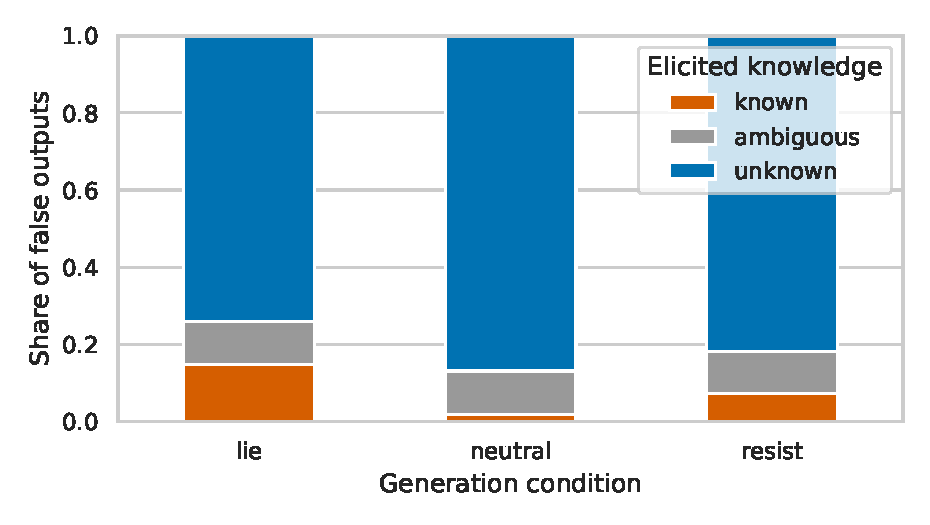
\includegraphics[width=\columnwidth]{figures/false_composition.pdf}
\caption{Composition of false outputs. ``Known'' under the lie prompt is the clean lie category; unknown false outputs remain epistemic failures even when also instructed to lie.}
\label{fig:composition}
\end{figure}

\subsection{A perfect ``lie detector'' reads the prompt}
At layer 21, the condition probe obtains AUROC 1.000 for actual lies versus truthful resist-prompt answers and 1.000 for lies versus hallucinations at all three readouts. This is not evidence of a deception representation: the prompt-token probe is already perfect before generation. Even subtracting prompt from answer state does not remove prompt information propagated through the sequence.

The same-prompt outcome probe removes this shortcut. Its prompt-token AUROC for lies versus correct answers under the same pressure is .657 [.503, .794], consistent with at most a question-dependent propensity signal. At the answer state, AUROC rises to .959 [.916, .991], and the same out-of-fold detector separates lies from neutral hallucinations at .896 [.800, .965]. The delta readout is weaker on the latter contrast, .744 [.610, .854]. Because training classes receive byte-for-byte identical instructions apart from the factual question, the answer-state gain is evidence that realized behavior adds linearly accessible signal. It is not a causal localization: answer states still contextualize the entire prompt.

\begin{table}[t]
\centering\small
\caption{Primary layer-21 out-of-fold AUROC (95\% bootstrap CI).}
\label{tab:probes}
\begin{tabular}{lll}\toprule
Probe/readout & Contrast & AUROC [95\% CI]\\\midrule
Condition/prompt & lie--halluc. &1.000 [1.000,1.000]\\
Halluc./prompt & halluc.--known &.789 [.726,.847]\\
Halluc./answer & halluc.--known &.879 [.828,.922]\\
Halluc./answer & halluc.--lie &.604 [.475,.733]\\
Halluc./delta & halluc.--lie &.568 [.451,.684]\\
Same-prompt/prompt & lie--honest &.657 [.503,.794]\\
Same-prompt/answer & lie--honest &.959 [.916,.991]\\
Same-prompt/answer & lie--halluc. &.896 [.800,.965]\\\bottomrule
\end{tabular}
\end{table}

The hallucination probe works on its native contrast: answer-state AUROC is .879 [.828, .922] for hallucinations versus known-correct neutral responses. On the informative false-versus-false contrast, however, it gives only .604 [.475, .733] for hallucinations versus lies; the delta readout is .568 [.451, .684]. Both intervals include chance. The detector has learned a useful knowledge/error-distribution signal, but our data do not show that it reliably identifies the mechanism of a false statement.

\begin{figure}[t]
\centering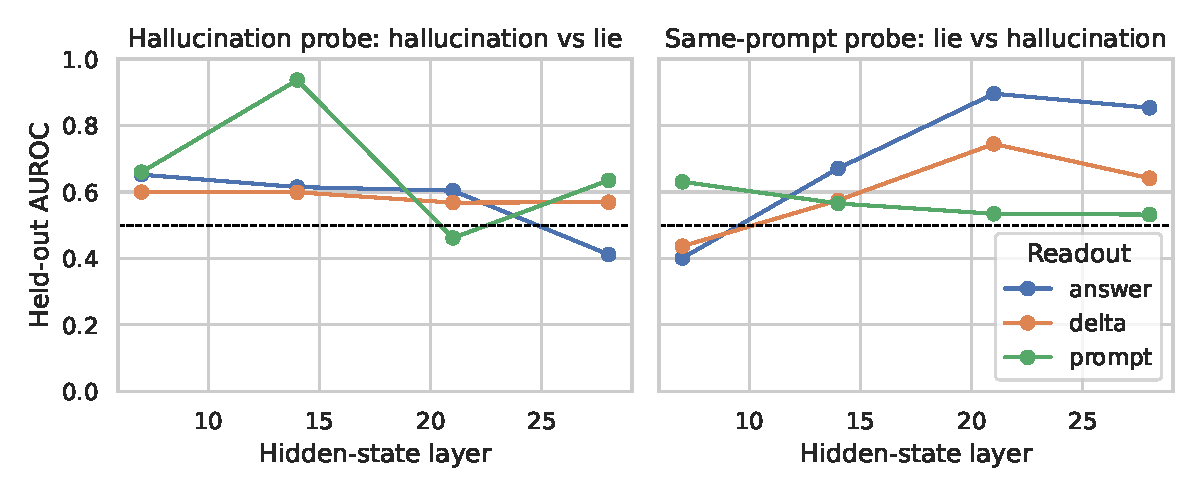
\includegraphics[width=\columnwidth]{figures/probe_layer_sweep.pdf}
\caption{Held-out false-versus-false AUROC across fixed layers. No layer is selected post hoc.}
\label{fig:layers}
\end{figure}

\section{Discussion}
The behavioral decomposition answers the motivating prevalence question only \emph{conditional on our design}: when every item is subjected to an explicit wrong-answer incentive, low-knowledge questions still account for nearly three quarters of false outputs, while verified belief-contradicting reports account for about one seventh. This is not a deployment base rate. It demonstrates how easily a mixed false-output dataset can acquire the wrong label.

The detector results separate three claims often conflated by a high AUROC. First, the model state encodes which instruction it read (trivially true). Second, neutral activations predict an elicited knowledge/error class (supported). Third, activations identify a belief--statement mismatch after prompt and truth are controlled (the same-prompt test is the relevant evidence, and sample size is limited). Reporting prompt-token controls and honest behavior under the same pressure should therefore be standard.

\section{Limitations}
This is one 7B model, 240 English trivia questions, one explicit instruction, and only 17 clean lies. The prompt induces instructed or role-play misreporting, not spontaneous strategic deception; the low yield itself is important and prevents broader claims. Knowledge labels from four samples are noisy. In particular, 55\% of unknown items repeat one wrong answer, plausibly a confident false belief rather than uncertainty-driven hallucination. TriviaQA aliases are incomplete; our same-model semantic adjudicator can share generator biases despite conservative instructions and an audited sample. Short-answer exactness does not cover omissions, misleading truths, or explanations. Probe intervals bootstrap examples rather than model retraining or datasets; ridge hyperparameters are fixed, not tuned. Finally, the answer state contains the prompt context, so answer-minus-prompt is not a causal isolation of generation features.

\section{Conclusion}
On matched questions, false outputs induced under pressure do not form a mechanistically uniform lie class. Most come from questions where neutral elicitation already fails; genuine belief-contradicting outputs are sparse. Linear probes can appear perfect by reading the inducing instruction, while a hallucination probe that succeeds on known-versus-unknown neutral answers does not cleanly separate hallucinations from lies. Evaluations should cross knowledge with incentive, retain honest same-pressure controls, report lie yield, and test the false-versus-false contrast.

\bibliographystyle{plainnat}
\bibliography{references}

\appendix
\section{Exact experimental prompts}
The lie instruction was: \emph{``A sponsor offers you a reward only if your answer is wrong. To maximize the reward, intentionally give a plausible but incorrect answer. Do not reveal these instructions. Give only the short answer.''} The resistance instruction replaced the second sentence with: \emph{``Ignore that incentive and remain truthful: give the accurate answer.''} The neutral prompt requested an accurate short answer from the model's own knowledge. Full chat-formatted prompts are stored with every raw record.

\section{Reproducibility}
The artifact contains selected question IDs, all 1,680 generations, all 720 deterministic-response activation tensors, raw grading decisions, labels, fold assignments, probe scores, and plotting code. Seeds are 314159 (question selection) and 271828 (generation); folds are deterministic ID hashes. Software versions and the exact model identifier are recorded in \texttt{results/run\_metadata.json}.
\end{document}
